\documentclass[../../../interview-questions.tex]{subfiles}

\begin{document}

\subsection{MySQL之InnoDB引擎的4大特性}

https://www.dounaite.com/article/627a65d1ac359fc91329676e.html

\paragraph{插入缓冲(Insert Buffer)}

插入缓存之前版本叫insert buffer,现版本 change buffer,主要提升插入性能,change buffer是insert buffer的加强,insert buffer只针对insert有效,change buffering对insert、delete、update(delete+insert)、purge都有效。有什么用呢?

对于非聚集索引来说,比如存在用户购买金额这样一个字段,索引是普通索引,每个用户的购买的金额不相同的概率比较大,这样导致可能出现购买记录在数据在数据里的排序可能是1000,3,499,35…,这种不连续的数据,一会插入这个数据页,一会插入那个数据页,这样造成的IO是很耗时的,所以出现了Insert Buffer。

Insert Buffer是怎么做的呢?MySQL对于非聚集索引的插入,先去判断要插入的索引页是否已经在内存中了,如果不在,暂时不着急先把索引页加载到内存中,而是把它放到了一个Insert Buffer对象中,临时先放在这,然后等待情况,等待很多和现在情况一样的非聚集索引,再和要插入的非聚集索引页合并,比如说现在Insert Buffer中有1,99,2,100,合并之前可能要4次插入,合并之后1,2可能是一个页的,99,100可能是一个页的,这样就减少到了2次插入。这样就提升了效率和插入性能,减少了随机IO带来性能损耗。

\paragraph{二次写(Double Write)}

在InnoDB将Buffer Pool中的Dirty Page刷(flush)到磁盘上时,首先会将(memcpy函数)Page刷到InnoDB System Tablespace的一个区域中,我们称该区域为Doublewrite Buffer(大小为2MB,每次写入1MB,128个页,每个页16k,其中120个页为后台线程的批量刷Dirty Page,还有8个也是为了前台起的sigle Page Flash线程,用户可以主动请求,并且能迅速的提供空余的空间)。在向Doublewrite Buffer写入成功后,第二步、再将数据分别刷到一个共享空间和真正应该存在的位置。

MySQL可以根据redolog进行恢复,而MySQL在恢复的过程中是检查page的checksum, checksum就是pgae的最后事务号,发生partial page write问题时. Dirty Page经损坏,找不到该page中的事务号就无法恢复。

\begin{figure}[htbp]
    \centering
    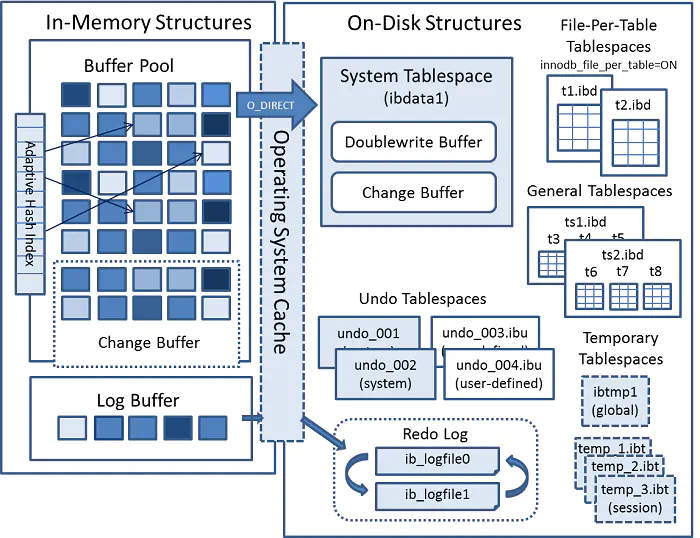
\includegraphics[scale=0.35]{innodbpng.png}
    \caption{InnoDB 8.0结构}
    \label{fig:innodbpng}
\end{figure}


\paragraph{自适应哈希索引(Adaptive Hash Index,AHI)}

哈希算法是一种非常快的查找方法,在一般情况(没有发生hash冲突)下这种查找的时间复杂度为O(1)。InnoDB存储引擎会监控对表上辅助索引页的查询。如果观察到建立hash索引可以提升性能,就会在缓冲池建立hash索引,称之为自适应哈希索引(Adaptive Hash Index,AHI)。

\paragraph{预读(Read Ahead)}

预读(read-ahead)操作是一种IO操作,用于异步将磁盘的页读取到buffer pool中,预料这些页会马上被读取到。预读请求的所有页集中在一个范围内。InnoDB使用两种预读算法:

Linear read-ahead:线性预读技术预测在buffer pool中被访问到的数据它临近的页也会很快被访问到。能够通过调整被连续访问的页的数量来控制InnoDB的预读操作,使用参数 innodb\_read\_ahead\_threshold配置,添加这个参数前,InnoDB会在读取到当前区段最后一页时才会发起异步预读请求
innodb\_read\_ahead\_threshold 这个参数控制InnoDB在检测顺序页面访问模式时的灵敏度。如果在一个区块顺序读取的页数大于或者等于 innodb\_read\_ahead\_threshold 这个参数,InnoDB启动预读操作来读取下一个区块。innodb\_read\_ahead\_threshold参数值的范围是 0-64,默认值为56. 这个值越高则访问默认越严格。比如,如果设置为48,在当前区块中当有48个页被顺序访问时,InnoDB就会启动异步的预读操作,如果设置为8,则仅仅有8个页被顺序访问就会启动异步预读操作。你可以在MySQL配置文件中设置这个值,或者通过SET GLOBAL 语句动态修改(需要有set global 权限)。

Random read-ahead: 随机预读通过buffer pool中存中的来预测哪些页可能很快会被访问,而不考虑这些页的读取顺序。如果发现buffer pool中存中一个区段的13个连续的页,InnoDB会异步发起预读请求这个区段剩余的页。通过设置 innodb\_random\_read\_ahead 为 ON开启随机预读特性。


\end{document}